% region preamble
\documentclass[11pt]{article}
\usepackage{import}
\usepackage[margin=1in, top=1in]{geometry}
\usepackage[all]{nowidow}
\usepackage[hyperfigures=true, hidelinks, pdfhighlight=/N]{hyperref}
\usepackage[separate-uncertainty=true, group-digits=false]{siunitx}
\usepackage{graphicx,amsmath,physics,tabto,float,amssymb,pgfplots,verbatim,tcolorbox}
\usepackage{listings,xcolor,subfig,caption,import,wrapfig,lipsum,tikz,biblatex,dirtree}
\usepackage[version=4]{mhchem}
\usepackage[noabbrev]{cleveref}
\newcommand{\creflastconjunction}{, and\nobreakspace}
\newcommand{\mb}[1]{\mathbf{#1}}
\newcommand{\pt}{p_\mathrm{T}}
\newcommand{\Cpp}{C\texttt{++}}
\numberwithin{equation}{section}
\numberwithin{figure}{section}
\numberwithin{table}{section}
\definecolor{stringcolor}{HTML}{C792EA}
\definecolor{codeblue}{HTML}{2162DB}
\definecolor{commentcolor}{HTML}{4A6E46}
\captionsetup{font=small, belowskip=0pt}
\definecolor{listinggray}{gray}{0.9}
\definecolor{Darkgreen}{rgb}{0,0.4,0}
\definecolor{lbcolor}{rgb}{0.9,0.9,0.9}
\lstset{
backgroundcolor=\color{lbcolor},
    tabsize=4,    
%   rulecolor=,
    language=[GNU]C++,
        basicstyle=\scriptsize,
        upquote=true,
        aboveskip={1.5\baselineskip},
        columns=fixed,
        showstringspaces=false,
        extendedchars=false,
        breaklines=true,
        prebreak = \raisebox{0ex}[0ex][0ex]{\ensuremath{\hookleftarrow}},
        frame=single,
        numbers=left,
        showtabs=false,
        showspaces=false,
        showstringspaces=false,
        identifierstyle=\ttfamily,
        keywordstyle=\color[rgb]{0,0,1},
        commentstyle=\color[rgb]{0.026,0.112,0.095},
        stringstyle=\color[rgb]{0.627,0.126,0.941},
        numberstyle=\color[rgb]{0.205, 0.142, 0.73},
%        \lstdefinestyle{C++}{language=C++,style=numbers}’.
}
\lstset{
    backgroundcolor=\color{lbcolor},
    tabsize=4,
  language=C++,
  captionpos=b,
  tabsize=3,
  frame=lines,
  numbers=left,
  numberstyle=\tiny,
  numbersep=5pt,
  breaklines=true,
  showstringspaces=false,
  basicstyle=\footnotesize,
%  identifierstyle=\color{magenta},
  keywordstyle=\color[rgb]{0,0,1},
  commentstyle=\color{Darkgreen},
  stringstyle=\color{red}
  }
\renewcommand{\lstlistingname}{Appendix}
\pgfplotsset{compat=1.17}
\addbibresource{bibliography.bib}
% endregion

\title{{\Huge A ``look-see'' at data from Run 3 at ALICE}}
\author{{\Large Miles Kidson}\\ \\
Supervisors: Prof. Zinhle Buthelezi, Dr. SV Fortsch, \& Prof. Tom Dietel\\
Assisted By: Dr. B Naik (Postdoctoral fellow)}
\date{\textbf{UCT Honours 2022}}

\begin{document}
    
\maketitle

\begin{figure}[h]
    \begin{center}
        
\includegraphics{Figs/UCT.jpg}
    \end{center}
\end{figure}

\begin{abstract}
    \centering
    We investigate pilot-beam data from proton-proton collisions in Run 3 at ALICE, checking if the new Muon Forward Tracker, Inner Tracking System, and Online-Offline analysis framework are working as intended. 
\end{abstract}

\newpage
\tableofcontents

\newpage
\section{Introduction}\label{sec:Introduction}
Run 3 is the latest period of data capture at the LHC, with an intended centre of mass energy per collision of $\sqrt{s}=\SI{13.6}{\tera\electronvolt}$ and increased luminosity of collisions---a factor 10 increase in integrated luminosity for Pb-Pb collisions. For Run 3, ALICE is moving from a triggered readout system to a combination of triggered and continuous readout. In order to achieve this, many detectors and their front-end electronics were upgraded, some new detectors were added, and the analysis framework was overhauled entirely. 

The Inner Tracking System (ITS) was upgraded with an entirely new pixel detector technology, hoping to greatly increase the resolution when determining the primary collision vertex. The Muon Forward Tracker (MFT) is one of the new detectors added. Its primary use is to assist the Muon Spectrometer (MCH) with vertexing and tracking in the forward region of ALICE and was developed with the same technology as the ITS. To deal with the increased volumes of data, a new analysis framework was introduced called Online-Offline (O2).

This report aims to use O2 to have a ``look-see'' at data coming from the ITS and MFT to see if the detector and analysis tools are working correctly. The data used in this investigation is from two proton-proton collision runs performed in October 2021, at a centre-of-mass energy of \SI{900}{\giga\electronvolt}. This is not an energy we expect to use for physics data analysis but is good enough for this purpose.

\section{Background}\label{sec:Background}
\subsection{The ALICE Detector}
\begin{itemize}
    \item What is the LHC?
    \item What is ALICE?
    \item What does ALICE look for?
    \item What is Run 3?
\end{itemize}
The ALICE detector (A Large Ion Collider Experiment) is a detector experiment at the Large Hadron Collider (LHC) at CERN. Its primary goal is the investigation of ``strongly interacting matter at extreme energy densities, where a formation of a new phase of matter, the quark-gluon plasma, is expected'' (\cite{ALICE_LOI}). It achieves this goal by studying the products of head-on collisions of heavy ions such as lead. 

% ALICE is situated at 

% The LHC at CERN in Geneva is built to accelerate particles up to very high energies (\SI{13.6}{\tera\electronvolt})

The coordinate system used at ALICE needs to be discussed first in order to fully explain the scope of this report. A modified cylindrical coordinate system is used as most detectors in the experiment are cylindrically symmetric about the beamline of the LHC. We place the $z$-axis along the beamline and call the angle around the $z$-axis $\varphi$, the azimuthal angle. The angle from the $z$-axis to the $x-y$ plane is called $\theta$, the polar angle. 
We are interested in the momentum of particles that we track in the detector, which we call $\vec{p}$, but we also define the transverse momentum $p_{\mathrm{T}}=\sqrt{p_x^2 + p_y^2}$. The last important coordinate to discuss is the rapidity, often denoted as $y$. This is defined as 
\begin{equation}
    y=\frac 12 \ln\left(\frac{E+p_z}{E-p_z}\right)
    \label{eqn:rapidity}
\end{equation}
where $E$ is the total energy of the particle being considered

\begin{figure}[h]
    \begin{center}
        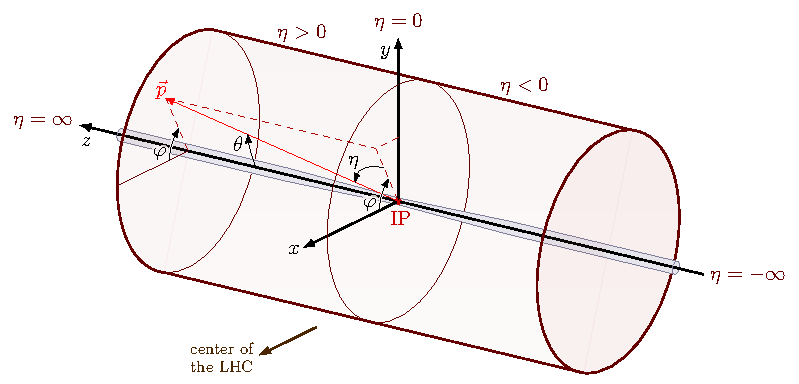
\includegraphics[width=.8\textwidth]{Figs/coords.pdf}
        \caption{Coordinate system \cite{coords}}
        \label{fig:coords}
    \end{center}
\end{figure}


\subsection{Run 3 Specifics}
\begin{itemize}
    \item What was upgraded/added in Run 3?
    \item 
\end{itemize}

\subsection{Muon Forward Tracker}

\section{Writing an Analysis Task}\label{sec:AnalysisTask}
Writing an analysis task in O2 is structured quite strictly, due to it needing to be run by O2. We will outline the steps needed to go from reconstructed data to histograms of, in our case, kinematic variables. It must be noted that learning how to do this, and how to deal with the idiosyncrasies of the O2 software, were what took up the majority of the time spent on this project. It is written to do one thing very very well, but unfortunately that comes with the side-effect of it being extremely picky about the conditions in which the software will actually work. 

\subsection{AOD Structure}\label{sec:AODStructure}
The data that we use in our analysis comes in the form of Analysis Object Data. These are in the form of ROOT files, which are based on a tree structure. In the tree are a number of tables corresponding to reconstructed tracks and collisions, among a few others. We call these entries or rows. For each of these tables, there are a number of reconstructed variables associated with each entry, such as their $\pt$, $\eta$, or $\varphi$, which we can access. There are 4 types of variables:
\begin{itemize}
    \item Static variables are saved to disk during the reconstruction process and are available at any time. $\varphi$ is a static variable.
    \item Dynamic variables are calculated on demand, using static variables as input. $\eta$ is a dynamic variable, calculated from $\theta$. 
    \item Index variables point from one table to another, such as from a track to its associated collision.
    \item Expression variables no clue
\end{itemize}

All variables associated with a track, for example, could be included in a single table. However, since we often only need a few of the variables, the tables are split up into sections that contain variables often used together. If needed, these tables can be joined together when doing analysis, using \lstinline[language=C++]{o2::soa::Join<Table1, Table2>}. Importantly, only tables which correspond row-to-row and have the same number of rows can be joined in this way.

\subsection{Analysis Task Structure}\label{sec:TaskStructure}
Analysis tasks are written in \Cpp and need to be structured in a specific way for O2 to use them properly. Each task is written as a \lstinline[language=C++]{struct} object which is then called at the end of the task. Below is an outline of what is needed for a task.

\begin{lstlisting}[language=C++]
#include "Framework/runDataProcessing.h"
#include "Framework/AnalysisTask.h"

struct MyTask {
    // Define things here, such as histogram registries, filters for 
    // data, or new tables

    void init{o2::framework::InitContext&} {
        // Here we initialise histograms and other things used in 
        // the analysis
    };

    void process(aod::Collisions const& collisions, aod::Tracks const& tracks) {
        // Here we can do any processing that we need, calculating 
        // things etc, and then fill the histograms we defined earlier
    };
};

//This
WorkflowSpec defineDataProcessing(ConfigContext const& cfgc)
{
  return WorkflowSpec{
    adaptAnalysisTask<MyTask>(cfgc),
  };
}

\end{lstlisting}


\newpage
\printbibliography

\end{document}


